\documentclass{beamer}
\usepackage{etex}
\usepackage{url}
\usepackage{semantic}
\usepackage{pgfpages}
\usepackage{multicol}\columnseprule 0.4pt
\usepackage{subfigure}
\usepackage{tikz,tikz-qtree}
\usepackage{verbatim,fancyvrb}
\usepackage{mathtools,mathrsfs,amsmath,amsthm,amsfonts}

%% Symbolic, relative link to thesis graphics.
\graphicspath{ {./pics/} }

%% Optional: Turn on Notes Pages:
\setbeameroption{show notes on second screen}

%% Beamer Theme Options
\usetheme{Rochester} % Because RIT.
\usecolortheme[named=black]{structure} % Default

%% Document Information:
\title{Process Cooperativity as a Feedback Metric \\
        in Concurrent Message-Passing Languages}
\author{Alexander Dean}
\institute{
    Rochester Institute of Technology\\
    Golisano College of Computer and Information Sciences
}
\date{August 12, 2014} % Scheduled Defense Date
\subject{Thesis Defense}

%% Document Table-Of-Contents, and pacing slides.
\AtBeginSection[]
{
    \begin{frame}
        \frametitle{Current Section:}
        \begin{multicols*}{2}
            \tableofcontents[sectionstyle=show/hide,
                             subsectionstyle=show/show/hide]
        \end{multicols*}
    \end{frame}
}

%% Slides have titles based on their section and subsection.
\newenvironment{slide}
    {\begin{frame}[environment=slide,fragile]
            \frametitle{\insertsection: \insertsubsection}
    }
    {\end{frame}}

%% Itemized Notes:
\newcommand{\inote}[1]{\note{\begin{itemize} #1 \end{itemize}}}

\begin{document}

% TITLE PAGE:
\frame{\titlepage
    \inote{
        \item Thank Fluet, Heliotis, and Raj.
        \item Dedicate to parents, who are unable to be present.
    }
}

% ToC PAGE:
\begin{frame}
    \frametitle{\centering
                Process Cooperativity as a Feedback Metric
                in Concurrent Message-Passing Languages}
    \begin{multicols*}{2}
        \tableofcontents
    \end{multicols*}
    \inote{
        \item Break apart title = Background.
        \item Then simulator and test primitives (process behaviours).
        \item Schedulers and how comparisons are made.
        \item Results, Conclusions (of both simulator and cooperativity).
    }
\end{frame}

% INCLUDE EACH SECTION:
\section{Background}

%%%%%%%%%%%%%%%%%%%%%%%%%%%%%%%%%%%%%%%%%%%%%%%%%%%%%%%%%%%%%%%%%%%%%%%%%%%%%%
\subsection{Runtime Scheduling}

\begin{slide}
    \begin{itemize}
        \item<1-> Schedulers can be defined in a discrete manner:
            \begin{enumerate}
                \item {\em Choose} a process from set,
                \item {\em Reduce} it,
                \item {\em Update} private scheduler state.
            \end{enumerate}
        \item<2-> Statistics can be gathered at every step about process:
            \begin{itemize}
                \item Timestamp of last run,
                \item Number of reductions, \etc
            \end{itemize}
        \item<3-> {\sl What statistics are useful?}
    \end{itemize}
    \inote{
        \item<2-> We can look at process schedulers like a function:
            \begin{itemize}{\scriptsize
                \item Takes a set of processes, and some private state.
                \item Job of the function is to choose a process, and run it for a bit.
                \item Then, based on what happened while running process, we update the state.
              }
            \end{itemize}
        \item<2-> Big questions: How are we choosing a process? What should effect our decision?
        \item<3-> Timestamp of last run? $\rightarrow$ 
            \begin{itemize}{\scriptsize 
                \item Choose always most recent, it's a batch scheduler.
                \item Choose oldest, we get something called Round-Robin.
                }
            \end{itemize}
        \item<3-> Number of reductions? $\rightarrow$ longevity = might want to 
                                                        give someone else a go.
        \item<3-> What are useful, and what do they tell us about the state of 
                the system? Well this leads us to cooperativity.
    }
\end{slide}


%%%%%%%%%%%%%%%%%%%%%%%%%%%%%%%%%%%%%%%%%%%%%%%%%%%%%%%%%%%%%%%%%%%%%%%%%%%%%%
\subsection{Cooperativity}

\begin{slide}
    What is Process Cooperativity?
    \begin{figure}
        \subfigure{
            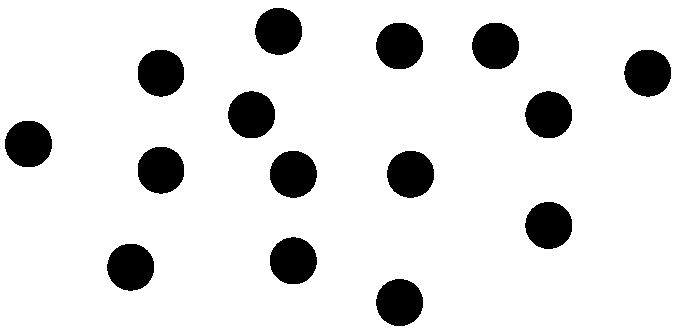
\includegraphics[scale=0.4]{ChugMachine.pdf}
        }
        \hspace{5mm}
        \rule{0.8pt}{4cm}
        \hspace{5mm}
        \subfigure{
            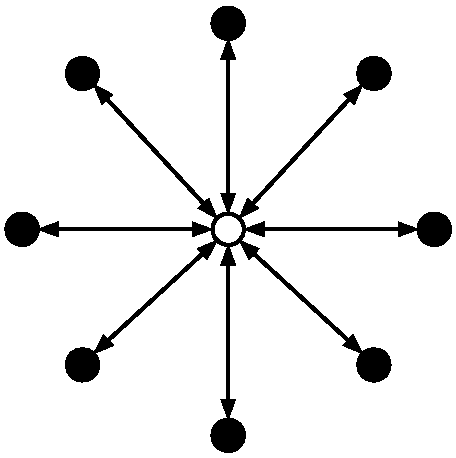
\includegraphics[scale=0.5]{SingleCluster.pdf}
        }
    \end{figure}

    \inote{
        \item What is Process Cooperativity?
        \item White = channel \& black = a process.
        \item Can think of channel a mechanism for passing information between processes. 
            \begin{itemize}
                \item These are nice functional abstractions of things like locks, shared-memory, \etc 
            \end{itemize}
        \item Left: Cloud of processes with no interaction.
        \item Right: We see a definite structure caused by some sharing of information.
              This is the core of recognizing cooperation, namely, recognizing these 
                structures when they exist.
    }
\end{slide}

\begin{slide}
    What does Cooperativity give us?
    \begin{figure} 
    \centering
        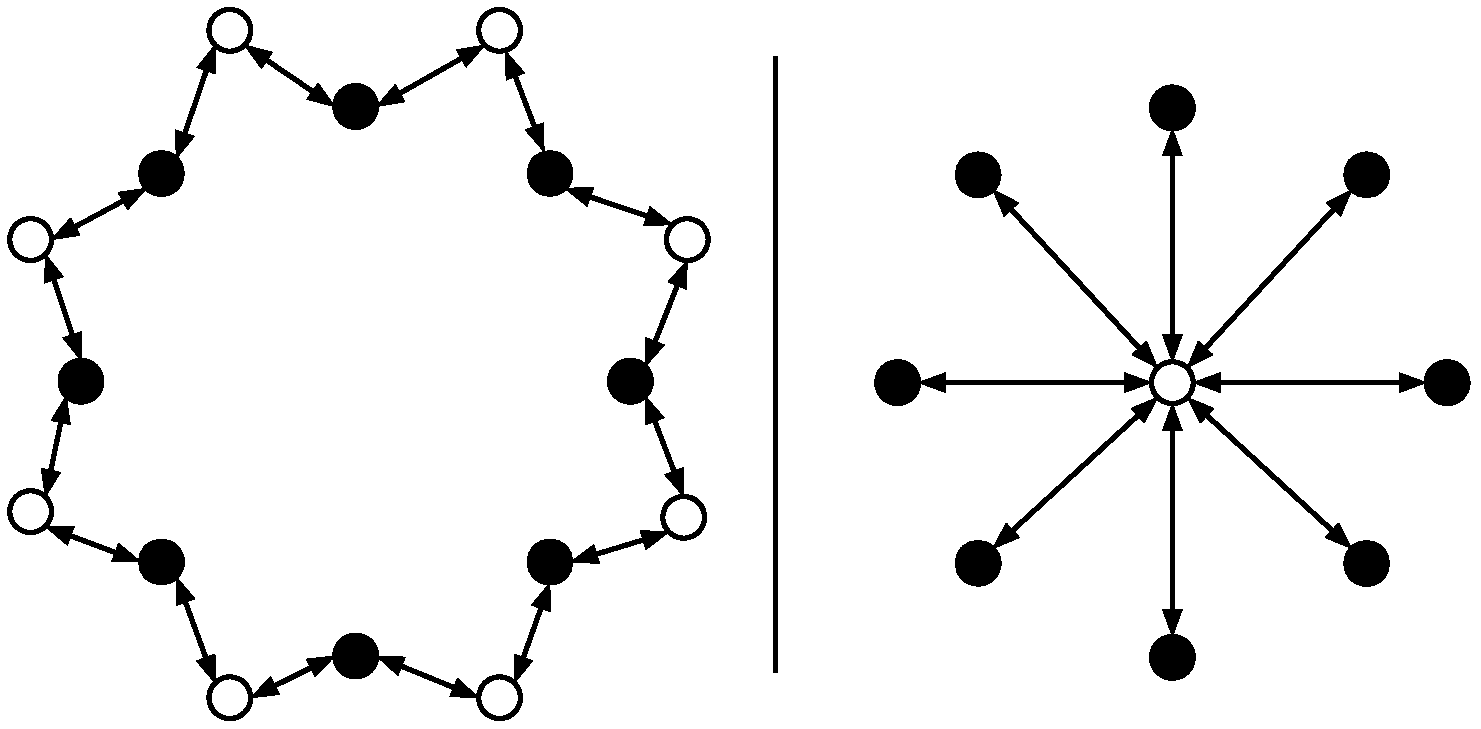
\includegraphics[scale=0.4]{RingVCluster.pdf}
        \label{fig:RingVCluster}
    \end{figure}

    \note{
        What does Cooperativity give us? \hfill
        What's the difference in the behaviour of cooperation in the left/right 
            applications?
        \begin{itemize}
            \item Left: A Ring, 
                \begin{itemize}{\scriptsize
                    \item the level of parallelism is nearly nil. 
                    \item Each process is cooperating yes, but granularity 
                        is very fine.
                    }
                \end{itemize}

            \item Right: A Star, 
                \begin{itemize}{\scriptsize
                    \item the level of parallelism is nearly full. 
                    \item Each process is cooperating,
                        {\bf not reliant on more than one} other process.
                    }
                \end{itemize}
            \item In both, the whole system is communicating, but with 
                cooperation, we can find the level of parallelism possible.
        \end{itemize}
        \hfill
        Next: Knowing this, how can we recognize cooperativity?
        Seems to be all about recording interactions with the channel.
    }
\end{slide}


%%%%%%%%%%%%%%%%%%%%%%%%%%%%%%%%%%%%%%%%%%%%%%%%%%%%%%%%%%%%%%%%%%%%%%%%%%%%%%
\subsection{Message Passing}

\begin{slide}
    We use a Symmetric, Synchronous, Message-Passing Primitive: 
            \begin{center} {\tt\large swap} \end{center}
    \begin{itemize}
        \item Purely captures cooperation of processes through synchronizing on
                a shared channel.
    \end{itemize}
    \inote{
        \item Symmetric, Synchronous, Message-Passing primitive.
        \item Symmetric:
            \begin{itemize}
                \item Only one message passing primitive: SWAP
            \end{itemize}
        \item Synchronous:
            \begin{itemize}
                \item Blocks until it's partner gets there.
            \end{itemize}
        \item Purely captures cooperation: Simple synchronization representation.
        \item This is really what I based the language on. 
        \item So, what does the rest of the language look like.
    }
\end{slide}



\section{ErLam}

\subsection{The Language}

\begin{slide}
    \begin{figure}
    \centering
        {\footnotesize
            %%
%% ErLam BNF Style Grammar.
%%
\begin{BVerbatim}[commandchars=\\\{\}]
<Expression> ::= <Variable> 
              |  <Integer>
              |  `\textbf{newchan}'
              |  `\textbf{(}' <Expression> `\textbf{)}'
              |  <Expression> <Expression>
              |  `\textbf{if}' <Expression> <Expression> <Expression>
              |  `\textbf{swap}' <Channel> <Expression>
              |  `\textbf{spawn}' <Expression>
              |  `\textbf{fun}' <Variable> `\textbf{.}' <Expression>
\end{BVerbatim}

        }
    \label{fig:grammer}
    \end{figure}

    \inote{
        \item Extremely simple on purpose (5 keywords).
        \item Issue now began to be how to build up test primitives
        \item Made a library which allowed for built ins.
    }
\end{slide}

\begin{slide}
    \begin{figure}
    \centering
    \begin{BVerbatim}
elib
    // ...
    omega = (fun x.(x x));
    // ...
    add = _erl[2]{ fun(X) when is_integer(X) ->
                        fun(Y) when is_integer(Y) ->
                            X+Y
                        end
                    end
                 };
    // ...
bile
    \end{BVerbatim}
    \end{figure}

    \inote{
        \item Theres options for built-ins as well as macros.
    }
\end{slide}

\begin{SaveVerbatim}[commandchars=\\\{\}]{FibCode}
// pfib.els -
fun N.
    (omega \textbf{fun} f,m.(
        \textbf{if} (leq m 1) 
           m
           (merge \textbf{fun} _.(f f (sub m 1))
                  \textbf{fun} _.(f f (sub m 2))
                  add)) \textit{N})
\end{SaveVerbatim}

\begin{slide}
\framesubtitle{Example Application: Parallel Fibonacci}
    \begin{figure}
    \centering
    {\small
        \BUseVerbatim{FibCode}
    } 
    \end{figure}
    \begin{itemize}
        \item[] {\tt els pfib.els} (Compile the script)
        \item[] {\tt ./pfib.ex -r 10} (Finds the 10th Fibonacci number)
    \end{itemize}
    
    \inote{
        \item R option is to run program applied to 10.
        \item To add more to this presentation than just reading paper
            I want to also give more detail as to system usage.
        \item Explain this Common Usage Pattern.
    }
\end{slide}

%%%%%%%%%%%%%%%%%%%%%%%%%%%%%%%%%%%%%%%%%%%%%%%%%%%%%%%%%%%%%%%%%%%%%%%%%%%%%%
\subsection{Channel Implementations}

\begin{slide}
    \begin{figure}
        \makebox[\textwidth][c]{
            \subfigure[t][Process Blocking Swap]{
                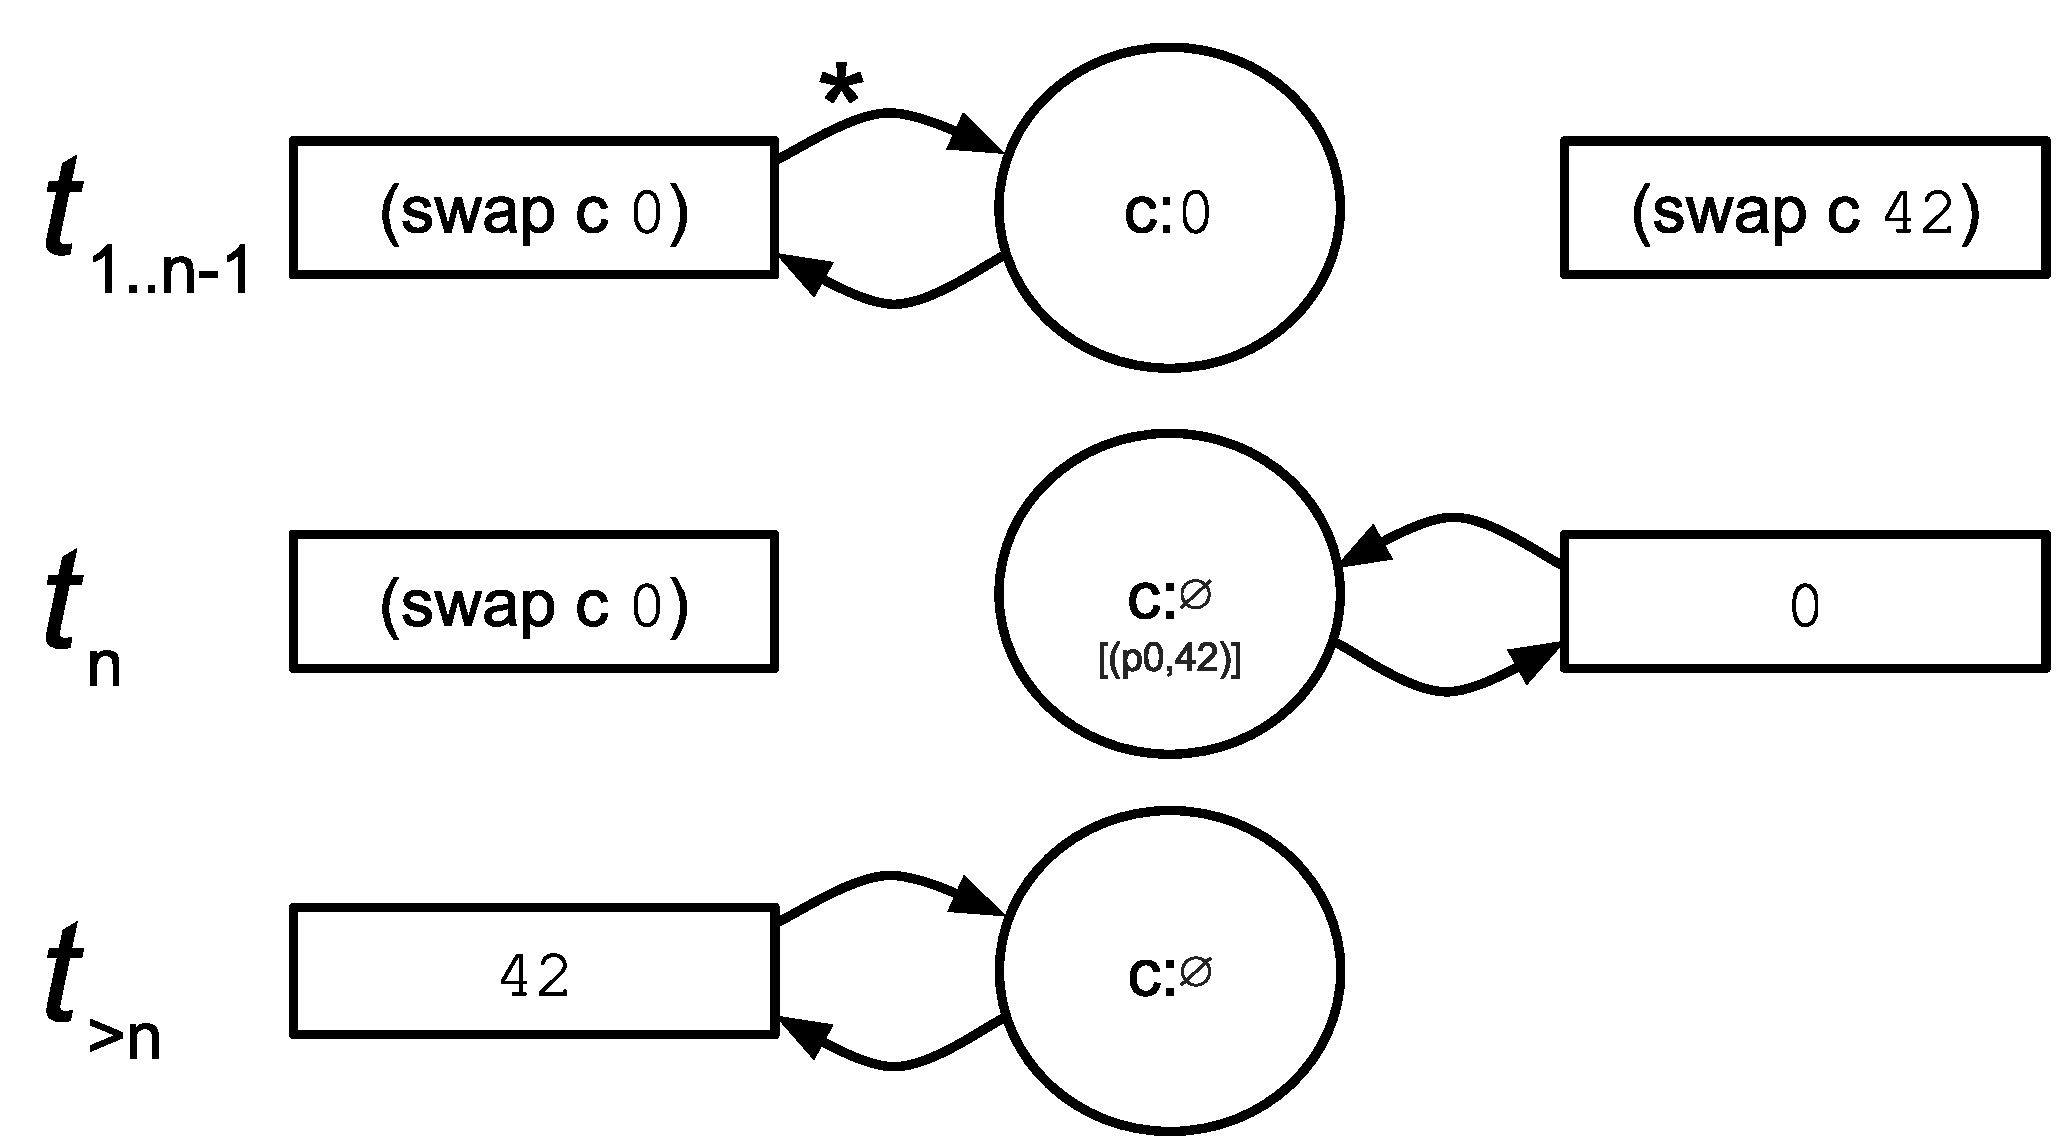
\includegraphics[width=0.5\textwidth]{BlockingSwap.pdf}
                \label{fig:blockchan-example}
            }  \subfigure[t][Process Absorption Swap]{
                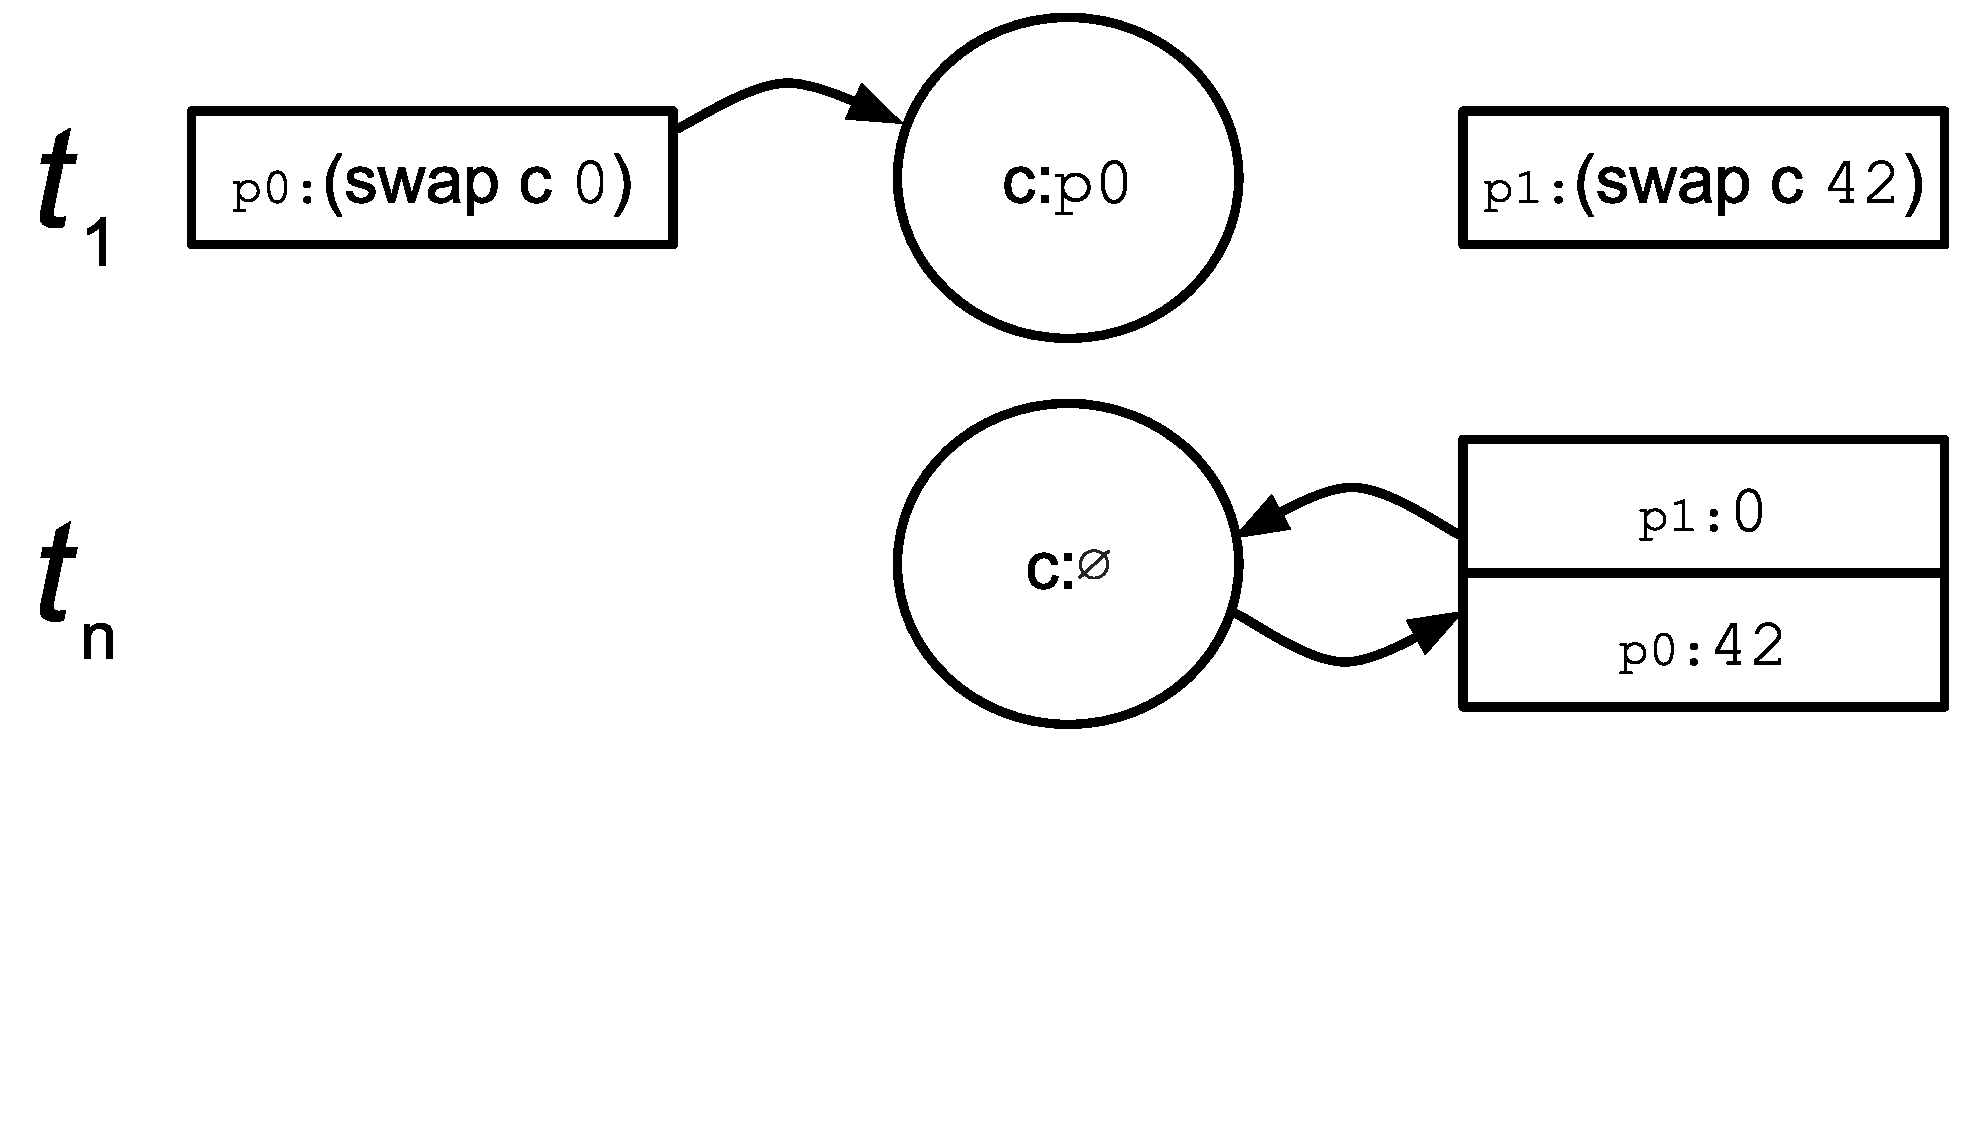
\includegraphics[width=0.5\textwidth]{AbsorbSwap2.pdf}
                \label{fig:absorbchan-example}
            }
        }
    \end{figure}
    \inote{
        \item Blocking: Maintains state of current and previous swap value until swap is completed.
        \item Absorption: Stores process which initializes the swap and returns it along with completion.
        \item Mention expected effects on scheduler.
        \item Blocking is default, passing '-a' to els 
    }
\end{slide}


%%%%%%%%%%%%%%%%%%%%%%%%%%%%%%%%%%%%%%%%%%%%%%%%%%%%%%%%%%%%%%%%%%%%%%%%%%%%%%
\subsection{Simulation \& Visualization}

\begin{slide}


    \inote{
        \item Need to talk about Chart types and chart generation.
    }
\end{slide}





















\section{Scheduler Implementations}

\subsection{Example Schedulers}

\begin{slide}
    \begin{itemize}
        \item Single-Thread Dual-Queue
            \begin{itemize}
                \item Translation of CML scheduler
            \end{itemize}

        \item Round-Robin with Single Global Queue (MTRRGQ)
            \begin{itemize}
                \item No Work-Stealing
                \item \# LPUs can vary
            \end{itemize}

        \item Round-Robin with Work-Stealing (MTRRWS)
            \begin{itemize}
                \item Steal via direct access
                \item Steal via advertisement
            \end{itemize}
    \end{itemize}

    \inote{
        \item First tested translating a known scheduler to the discrete step scheduler semantics.
        \item MTRRGQ: all synchronization around a single global queue, test P=1 or max.
        \item MTRRWS-SQ:
            \begin{itemize}
                \item Schedulers can access a random LPU's queue end and steal from their bottoms.
            \end{itemize}
        \item MTRRWS-IS:
            \begin{itemize}
                \item Uses a secondary queue to advertise desire to steal. 
                \item Scheduler can check secondary queue as desired.
                \item No requirement for synchronization on private process queue.
            \end{itemize}
    }
\end{slide}

\subsection{Feedback Schedulers}

\begin{slide}
    Three types of mechanics:
    \begin{itemize}
        \item Longevity-Based Batching
        \item Channel Pinning
        \item Bipartite-Graph Aided Sorting
    \end{itemize}

    \inote{
        \item Instead of a single cooperativity-conscious scheduler,
            we implemented three mechanics which take cooperativity into
            account on top of the basic schedulers.
   }    
\end{slide}

\begin{slide}
    \framesubtitle{Longevity-Based Batching}

    \begin{itemize}
        \item Choose via Round-Robin 
            \begin{itemize}
                \item from batch rather than queue
                \item keeps track of number of rounds (batch size)
            \end{itemize}

        \item Work-Steal whole batches

        \item Spawn to batch unless: $|b_i| \geq B$
            \begin{itemize}
                \item Make singleton with new process.
                \item Push parent and child into new batch.
            \end{itemize}

        \item[GOAL:]<2-> Can batching based on longevity account for fine/coarse
            parallelism in application? 

     \end{itemize}    
    
    \inote{
        \item Batching processes based on longevity.
            \begin{itemize}
                \item Based on occam-$\Pi$.
                \item if a process communicates frequently then
                    it will be batched (absorption), singleton if 
                    very computation-bound.
            \end{itemize}
        \item We are normal RR but with one extra layer.
        \item If batch is too big during spawns we can:
            \begin{itemize}
                \item Make singleton, best if child is needed to 
                    start work right away. Map-Reduce.
                \item Make push-back, parent can get another chance
                    to spawn more children sooner.
            \end{itemize}
    }
\end{slide}

\begin{slide}
    \framesubtitle{Channel-Pinning}

    \begin{itemize}
        \item Upon call to $newchan$, pin to LPU based on spread algorithm:
            \begin{itemize}
                \item $same$ - LPU $newchan$ is called is where it is pinned.
                \item $even$ - Cycle through LPUs and pin based on that.
                \item \ldots
            \end{itemize}

        \item Work-steal based on channel that's been pinned to you.

        \item[GOAL:]<2-> Can an $even$-like spread increase early saturation?
    \end{itemize}

    \inote{
        \item Pin channels to LPUs.
            \begin{itemize}
                \item Pinning a channel means to set a process affinity to a 
                      LPU based on the channels it uses.
                \item Work-Stealing works like Go-Fish.
            \end{itemize}
    }
\end{slide}


\begin{slide}
    \framesubtitle{Bipartite-Graph Aided Sorting}
   
    \begin{multicols*}{2} 
        \begin{itemize}
            \item Based on Round-Robin \& Work-stealing
            \item Keep track of events which may effect cooperativity:
                \begin{itemize}
                    \item Spawning
                    \item Blocking/Unblocking
                    \item Steals
                \end{itemize}
            \item If number of events over some threshold, re-sort. 
        \end{itemize} 
    
        \begin{figure}
            \centering
            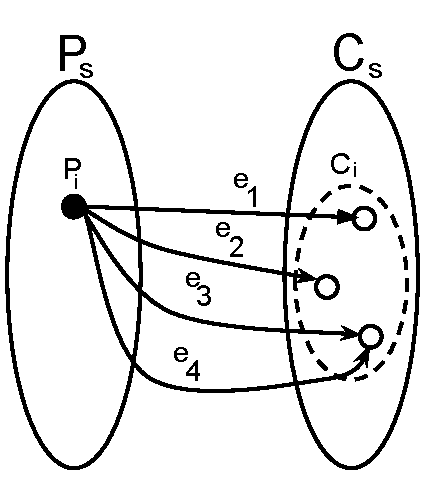
\includegraphics[scale=0.5]{BipartiteGraph.pdf}
            \vspace{5mm}
        \end{figure}
    \end{multicols*}

    \begin{itemize}
        \item[GOAL:]<2-> Are alternate channel implementations worth exploration?
    \end{itemize}

    \inote{
        \item Keep a list of all communications as a graph between set of processes and channels.
    }
\end{slide}


\section{Results}

\begin{slide}
    Longevity-Based Batching Scheduler:
    \begin{itemize}
    \item Spawn Mechanism 
    \item[] ~~~~{\it (Where does a new process go if batch is too big?)}
    \end{itemize}
    
    Channel Pinning Scheduler:
    \begin{itemize}
    \item Channel Spread 
    \item[] ~~~~{\it (How to spread the channels across processors?)}
    \end{itemize}

    Bipartite-Graph Aided Sorting Scheduler:
    \begin{itemize}
    \item Channel Implementation 
    \item[] ~~~~{\it (Does blocking help to take advantage of sorting?)}
    \end{itemize}

    \inote{
        \item LBB: Can also look at how the batch size effects different types
            of behaviours.
        \item SS: Could also look at a stealing mechanism.
    }
\end{slide}

\begin{slide}
\framesubtitle{Longevity-Based Batching Scheduler}

        \begin{table}[htp!]
            \centering
            \begin{tabular}{@{}cccc}
                & \multicolumn{3}{c}{$PRing_N$} \\ \cline{2-4}
            & $N=P=8$ & $N=B=10$ & $N=2*B=20$     \\ \cline{2-4} 
                \multicolumn{1}{c|}{\rotatebox{90}{\rlap{\textbf{Reduc. Density}}}} & 
            \multicolumn{1}{c|}{\includegraphics[scale=0.15]{tests/pring/longbatcher/8/pg_0004.pdf}} & 
            \multicolumn{1}{c|}{\includegraphics[scale=0.15]{tests/pring/longbatcher/10/pg_0004.pdf}} & 
            \multicolumn{1}{c|}{\includegraphics[scale=0.15]{tests/pring/longbatcher/20/pg_0004.pdf}} \\ 
            \cline{2-4} 
        \end{tabular}
        \caption{Comparison of different sized $PRing_N$ on the Longevity 
                 Batching Scheduler with batch size $B=10$.}
            \label{tab:pring-longbatcher-testing}
        \end{table}

    \inote{
        \item Before talking about spawn mechanism, pointing out the
              primary goal and effect of batching to catch the granularity
              of the application.
    }
\end{slide}
\begin{slide}
\framesubtitle{Longevity-Based Batching Scheduler}
    \inote{
        \item TODO: Get simple $ClusterComm_{(N,1)}$ or the PTree results to contrast with PRING 
        \item This brings it back to an issue of behaviour recognition.
    }
\end{slide}


\begin{slide}
\framesubtitle{Channel Pinning Scheduler}
    \begin{table}
    \centering
    \begin{tabular}{@{}ccc}
    & \multicolumn{2}{c}{$Interactivity_{(20,0)}$} \\ \cline{2-3} 
    & \multicolumn{1}{c}{$MTRRWS$-$SQ$}       & \multicolumn{1}{c}{Channel Pinning} \\ \cline{2-3} 
 
    \multicolumn{1}{c|}{\rotatebox{90}{\rlap{~~Queue Length}}} &
    \multicolumn{1}{c}{\includegraphics[scale=0.15]{tests/interactivity/20/wssq/ca/pg_0003.pdf}} & 
    \multicolumn{1}{c|}{\includegraphics[scale=0.15]{tests/interactivity/20/cp/ca/pg_0003.pdf}} \\

    \multicolumn{1}{c|}{\rotatebox{90}{\rlap{Reduc. Density}}} &
    \multicolumn{1}{c}{\includegraphics[scale=0.15]{tests/interactivity/20/wssq/ca/pg_0004.pdf}} & 
    \multicolumn{1}{c|}{\includegraphics[scale=0.15]{tests/interactivity/20/cp/ca/pg_0004.pdf}} \\ \cline{2-3}
    \end{tabular}
    \label{tab:cp-compare-rand-uniform-ca}
    \end{table}

    \inote{
        \item Comparison of Uniform synchronization for $MTRRWS$-$SQ$ 
                and the Channel Pinning Scheduler on Absorption Channels.
        \item This used the $even$ spread type.
        \item Note the speed at which it saturates all cores.
        \item Despite Naive WS, we still have decent spread.
    }
\end{slide}

\begin{slide}
\framesubtitle{Bipartite-Aided Graph Sorting Scheduler}

    \begin{table}
    \centering
    \begin{tabular}{@{}ccc}
        & \multicolumn{2}{c}{Parallel Fibonacci} \\ \cline{2-3}
        & $MTRRWS$-$SQ$ & Sorting Scheduler  \\ \cline{2-3} 
        \multicolumn{1}{c|}{~}  & 
        \multicolumn{1}{c|}{\includegraphics[scale=0.27]{tests/pfib/wssq/pg_0001.pdf}} & 
        \multicolumn{1}{c|}{\includegraphics[scale=0.27]{tests/pfib/ss/pg_0001.pdf}} \\ \cline{2-3}
    \end{tabular}
    \label{tab:ss-compare-fib}
    \end{table}

    \inote{
        \item Channel State comparison of Parallel Fibonacci executed on 
                $MTRRWS$-$SQ$ and the Bipartite-Graph Aided Sorting Scheduler. 
        \item Note the large reduction in number of ticks.
    }
\end{slide}


\section{Conclusions \& Future Work}

\subsection{ErLam Toolkit}

\begin{slide}
    \begin{itemize}
        \item Test Primitives were nicely composable process behaviours.
            \begin{itemize}
                \item More research into generating behaviours.
                \item More compositions: PTree with Rings.
            \end{itemize}

        \item Log generation, lots of overhead, but good observations.
    \end{itemize}

    \inote{
        \item Overall pleased with simulator and achieved its goal.
        \item Future Work: 
            \begin{itemize}
                \item Generate more test primitives, a good library of them 
                        would be nice.
                \item Compose them easier and more frequently. Perhaps 
                    generating work groups as PRing might have made a better 
                    comparison than Interactivity.
 
                \item Clean up log generation (reduce overhead).
                \item Process evaluation uses alpha-reduction 
                      (can be sped up substantially).
                \item Make schedulers more adjustable (different
                        spawn/yields/etc).
                \item More Channel implementations
            \end{itemize}
    }
\end{slide}

\subsection{Cooperative Schedulers}

\begin{slide}
    \begin{itemize}
        \item {\bf Longevity Batching:}
            \begin{itemize}
                \item Would benefit from heuristic based Quantum selection.
                \item As it stands, limited gain from longevity recognition.
                \item[] ~
            \end{itemize} 
        \item {\bf Channel Pinning:}
            \begin{itemize}
                \item Promising saturation and work-stealing mechanic.
                \item[] ~
            \end{itemize}
        \item {\bf Bipartite-Graph Aided Sorting:} 
            \begin{itemize}
                \item Supprising results on MapReduce style applications.
                \item Worth studying Blocking-Channels further for gains from 
                    sorting.
            \end{itemize}
    \end{itemize}

    \inote{
        \item SS: Would benefit from merging with Channel Pinning. Increase 
            likelihood that sorting puts channel partners close.
    
        \item LBB + CP might be interesting as channels could own batches.

        \item Overhead of Sorting? If implemented in a practicle language,
            would it be worth it? Seems counter-intuitive but promising as is.
    }
\end{slide}

\subsection{Cooperativity as a Metric}

\begin{slide}

    \begin{itemize}
        \item Possible to recognize and benefit from.
        \item The three example mechanics are promising and can be extended for
                practicle modern languages, despite simplistic simulation language.
        \item More to explore:
            \begin{itemize}
                \item Alternate Message-Passing Types (Asymmetric?)
                \item \ldots
            \end{itemize}
    \end{itemize}

    \inote{
        \item Promising scheduling mechanics
        \item More research is necessary in the message-passing implementation
                for it to be practical in common languages.
        \item (Asymmetric/Directionality would be first on the list)
    }
\end{slide}




% Questions and Thank you!
\section*{Questions}
\begin{frame}
    \begin{center}
        {\Huge Questions/Comments?}
    \end{center}

    \uncover<2->{
        \begin{center}
            Thank You!
        \end{center}
    }
\end{frame}

% Bibliography and Links Sections:
%\input{sections/999bibliography}
\begin{frame}
    \frametitle{Links:}

    \begin{itemize}
        \item \url{https://github.com/dstar4138/erlam}
        \item \url{https://github.com/dstar4138/thesis_cooperativity}
        \item \url{http://dstar4138.com}
    \end{itemize}
\end{frame}


\end{document}
